\documentclass{article}
\usepackage[utf8]{inputenc}
\usepackage[portuguese]{babel}
\usepackage{csquotes}
\usepackage{graphicx}
\usepackage{adjustbox}
\usepackage{lipsum}
\usepackage[backend=biber,autolang=other,
  bibencoding=utf8,style=alphabetic,
  ibidtracker=true]{biblatex}
\addbibresource{holanda.bib}

\title{A Ciência do Desenho de Franscisco da Holanda} \date{20 de
  Abril de 2015} \author{João Távora \\Faculdade de Belas Artes da
  Universidade de Lisboa}

\begin{document}

\maketitle

\section{Sinopse}

\section{Palavras-chave}

Holanda, Idade Média

\section{Introdução}

Francisco da Holanda escreve o livro ``A ciência do Desenho'' em 1571
e dedica-o, no próprio extensíssimo título da obra, a El-Rei
D. Sebastião como ``lembrança ao sereníssimo e cristianíssimo Rei
[...] de quanto serve a ciência do Desenho [...]  assim na paz como na
guerra''.

Esta obra ``A ciência do Desenho'', como é frequentemente abreviada,
estrutura-se de forma simples em 7 pequenos capítulos. Introduzida no
prólogo a motivação da escrita, os primeiros capítulos procuram ser um
levantamento, em jeito de alerta, dos avanços verificados pelos outros
reinos, e do isolamento de Portugal, naquela que se tornava cada vez
mais uma arte respeitada, a pintura.

Estabelecida a urgência e pertinência da lembrança, o segundo capítulo
apresenta uma concepção inovadora e enaltecedora do ``DESENHO''
enquanto actividade intelectual, contrastando-a com o ``debuxo''
associado à simples prática manual. Os capítulos seguintes enumeram
sistematicamente a utilidade aplicada do desta ciência nos diversos
contextos práticos que o autor considera que possam interessar
directamente a El-Rei.

Assim, o Desenho é útil, por esta ordem, no serviço Deus, à pessoal
real, na paz e na guerra. 

Na dimensão, a obra é assumidamente pequena, como é directamente
assumido no título do último capítulo ``Conclusão desta pequena
obra''.

Francisco da Holanda ilustra amplamente as suas ideias com episódios
da sua própria experiência profissional de arquitecto, bem como alguma
evidência anedótica de difícil verificação. As referências
auto-bibliográficas são tão numerosas que, na edição consultada
(\cite{holanda}), José da Felicidade Alves, se inclui até uma seçcão
exclusivamente dedicada a enumerá-las, contando-se em certas páginas
do manuscrito original mais de uma dezena delas.

\section{O queixume e os ``outros reinos''}

As primeiras duas palavras da obra do Prólogo d' ``A Ciência do
Desenho'' são ``Um queixume'':

\begin{quote}
  Um queixume faz por mim a Arte da Pintura a Vossa Alteza [...], de
  quão pouco ]e bem entendida e estimada, neste vosso Reino de
    Portugal, sendo uma ciência e arte digníssima [...] E somente em
    portugal não é conhecida nem tem o resplendor e lustro que merece.
\end{quote}

Mais adiante, Holanda esclarecerá que não é por ``ressábio'' que se
queixa \cite[fl.36v]{holanda}, mas pela benévola motivação de alertar
o mais alto responsável do Reino de como periga o futuro do reino se
não se compreenderem e promoverem devidamente as artes.

O leitor d'``A ciência do Desenho'' depara-se por toda a obra com uma
marcação deliberada da autoridade do autor, sobretudo referências aos
trabalhos realizados por Holanda aos antepassados de D. Sebastião, bem
como referências ao seu próprio pai, António Dolanda que seria
protegido do imperador Carlos V.

Assim, no primeiro capítulo Holanda começa por estabelecer a amplitude
do seu conhecimento na matéria \cite[fl.34r]{holanda}:

\begin{quote}
  [...] porque as li, e vi e sei e tratei [...] que me atrevera a
  encher muitos livros [...]
\end{quote}

Afirma novamente a brevidade da presente obra, e que tratará nela
apenas de uma pequena fracção da centena de pintores e artistas que
conheceu e admira.

\begin{quote}
  [...] haver piedade dela e dos que não entendem o preço de tão
  ilustríssima ciência, determinei de escrever este breve caderno
  acerca do valor que tem a Arte do Desenho da Pintura na República
  Cristã assim no tempo da paz como no tempo da guerra.
\end{quote}

Segundo Holanda, a pintura (e a do Desenho, como virá a pretender) tem
``origem divina'', e por essa razão, sempre foi muito estimada por
``todas as repúblicas famosas e regidas com policia não bárbara''.

A pintura e o Desenho, neste ponto do livro ainda indistintos, são
enquadrados numa moldura divina e com certa complexidade
mística \footnote{É plausível que a formulação algo retorcida desta
  frase tenha provindo da ``censura benévola'' de Frei Bartolomeu
  Ferreira, ainda que esta folha não apresente as emendas encontradas
  noutras folhas por José da Felicidade Alves.}. Afirma-se que estas
artes ``deriva[m] de [S]ua eterna origem a ideia dalgum grande engenho
no entendimento'' \cite[fl.34r]{holanda}. Uma vez estabelecida no
plano transcendental, a ideia da eternidade é repetido no plano
político já que o Desenho ``em todas as idades e nações do mundo
sempre foi e é hoje muito estimado'' \cite[fl.34r]{holanda}

Entre ``outros reinos'' eleitos como exemplos, citam-se os de
Alexandre, de Antíoco, e o de César. Citam-se os pintores Protógenes e
Apeles \footnote{Crê-se que o elogio ao pintor Apeles provinha
  totalmente da celebridade do mesmo, já que deste não se conhece
  nenhuma obra em concreto. \cite{calado}} e Panfilo, preocupando-se
em enquadrar as relações privilegiadas que estes artistas mantinham
com os seus soberanos. Neste ponto, Holanda faz questão de refutar que
apenas os antigos, ``gentios e pagãos'' se preocupariam com as artes,
estabelecendo a ligação com a época cristã. Refere Leonardo da Vinci ,
que terá morrido nos braços do Rei de França, bem como as as ligações
de Rafael e Miguel Ângelo com o papado.

Esta folha d'``A Ciência do Desenho'' ilustra a lado lúdico e
anedódito da obra: quanto a Rafael, refere-se uma
historieta \footnote{Colhida nas ``Vidas'' de Vasari, segundo José da
  Felicidade Alves, em nota da edição, e portanto de fiabilidade
  relativa. } segundo a qual Rafael se teria mantido solteiro na
esperança que o papa o fizesse cardeal. Já de Miguel Ângelo, que
Holanda estimava particularmente e com quem teria mantido contacto
pessoal, conta-se a anedota ainda mais bizarra de que o pintor,
célebremente irascível, ``tirou quase uma tábua que houvera de
escalavrar o Papa'' quando se sentiu desrespeitado no seu estúdio.

\section{O Desenho como ideia}

É notória em toda a obra a insistência e prevalência do termo
``ciência'' a preceder ``Desenho'' e ``Pintura'', ora só, ora
emparelhado com ``arte'', ou seja, Holanda esforça-se desde o início
para fazer descolar estes termos das ideias de manualidade e
artesanato. Ainda assim, no segundo capítulo da obra de Holanda que
reside e se desenvolve o núcleo teórico da obra, a definição inovadora
do ``Desenho'' como ideia e actividade intelectual.

\begin{quote}
  E digo que a Pintura ou debuxo de que trato não é o que comummente
  se chama debuxar ou pintar, dos que pouco sabem; qual é o ofício dos
  que debuxam lavores e folhagens, ou dos que pintam com tintas
  vermelhas e azuis de verdes (em quanto terra) porque deste debuxar e
  pintar eu aqui não falo. Mas escrevo daquela ciência, não só
  aprendida por ensino doutros pintores: mas naturalmente dada por o
  sumo mestre Deus gratuita no entendimento, procedida de sua eterna
  Ciência, a qual se chama DESENHO, e não debuxo nem pintura. O qual
  Desenho, assim natural do entendimento por Deus [...] é uma coisa
  tão grande e um dote tão divino, que o mesmo que Deus obra nele
  naturalmente, obra ele em todas as obras, manuais e intelectuais,
  que podem ser feitas ou imaginadas.
\end{quote}

Neste parágrafo reconhece-se, por um lado, a reprodução da estrutura
neo-platónica das artes e a distinção entre material e intelectual.

Por outro lado, Holanda revela considerável habilidade em entretecer a
sua concepção de Desenho nesta mesma estrutura: O novo conceito de
``Desenho'' é efectivamente distinto da sua componente material,
confusa, suja e terrena, e é investido de uma leveza e uma
constituição apriorística que transcende qualquer outra actividade,
para se afirmar como a linguagem com que o próprio Deus ``obra
naturalmente [...] em todas as obras, manuais e intelectuais, que
podem ser feitas ou imaginadas''.

A manisfestação humana do Desenho de Holanda é exclusivamente
intelectual, e é ``incriada'' na nossa ciência a partir da sua origem
eterna. É assim que se dá origem a todas as obras. É a Deus, e não aos
artistas \footnote{Neste ponto, Holanda ousa colocar-se ao lado de
  Apeles e Miguel-Ângelo como ``presuntuosos''. Segundo José da
  Felicidade Alves, nas notas da edição consultada, trata-se de uma
  figura de estilo. É possível que Holanda tenha decidido investir
  nela de forma assegurar a passagem da ideia principal pelo crivo da
  censura. Segundo o editor, a folha original apresenta várias emendas
  de ``censura benévola'' do Frei Bartolomeu Ferreira, particularmente
  nas formulações em que intervém directamente a divindade. O mesmo
  frade declara no final na folha ``já isto está emendado''} que nelas
trabalharam, que redunda a toda a glória pela criação dessas obras.

Os parágrafos seguintes são ainda mais claros, colocando o Desenho
como actividade primeira e identificando-o totalmente à Ideia
platónica. O Desenho está pre-constituído em toda as actividades
criadoras, não só na produção de imagens através da
pintura. \footnote{Em \cite{teresa}, Teresa Lousa formula que o
  Desenho é, para Holanda, ``uma categoria absolutamente Universal
  [...] presente tanto na mais pura especulação filosófica, como na
  execução de uma obra de arte''.}

\begin{quote}
  De que vem dizerem também que os Imperadores na guerra que têm
  desenho de ir assentar o seu campo em tal província, ou de combater
  com seu exército tal cidade ou de fazer tal fortaleza, muito antes
  que o façam, tendo feito já o desenho na deliberação secreta do
  entendimento.
\end{quote}\cite[fl.37v]{holanda}

Fica deste modo claro a equivalência de ``Desenho'' a ``desejo'':
todas as criações de Deus são ``interiores nas ideias, como exteriores
na obra''\cite[fl.37v]{holanda}. \footnote{Foi historiador Robert
  Klein que faz notar, já no séc. XX que a coincidência destas ideias
  com Federico Zuccaro, que por volta de 1600 viria a cunhar os termos
  ``Disegno interno'' e ``Disegno Externo'' é praticamente total, e
  que só pode ter sido holanda a desenvolvê-las antes dos seus
  contemporâneos e, muito provavelmente, independentemente deles}.

\section{Serviço a Deus, paz e guerra }

Os capítulos intermédios d'``A ciência do Desenho'' consistem, em
grande medida, na enumeração da diversas utilidade práticas do Desenho
em quatro categorias: o ``serviço de Deus'', o ``serviço de El-Rei'',
``em tempo de guerra'' e no ``real ornamento''.

O ``serviço de Nosso Senhor, que é o principal''\cite[fl.38r]{holanda}
figura em primeiro lugar. O desenho serve para ``fazer a feição do
cálix em perfeita proporção'', ``iluminar de ouro as letras da
Sacra'', ``em as images dos livros iluminados'', ``para a forma e
feição dos sacrários e custódias'', etc, etc...

Muitos destes exemplos são complementados com referências à própria
experiência, ou à do pai, António Dolanda, que trabalhou para
D. Manuel, bisavô de D. Sebastião.

Nas críticas mais ou menos explícitas, Holanda parece falar
directamente ao fervor religioso que acompanhava a ascenção de
D. Sebastião ao trono:

\begin{quote}
  [...] não corrompendo confusamente a Arquitectura, como se faz em
  algumas partes, não fazendo entalhos nem pinturas indiscretas e mui
  pouco para estar em altar, que muito se deve advertir dos Bispos
  [...] 
\end{quote}

O capítulo termina com mais uma formulação que, sendo tipicamente
neo-platónica, possui uma impressionante poesia, recorrendo à
simbólica da descobertas:

\begin{quote}
  Serve sobretudo o Desenho de levantar o espírito a Deus, pelas
  coisas visíveis às invisíveis, vendo o mundo e o mar e o céus, como
  olhos mais claros que outros em sua pintura.
\end{quote}

No 4º capítulo, a enumeração prossegue na mesma lógica: o Desenho
serve a El-Rei no ``ceptro do seu reino, como fez meu pai'', ``na
coroa real'', ``na invenção das divisas'', etc... Este é o capítulo do
``tempo de paz'' e termina com a introdução do seguinte capítulo.

\begin{quote}
  Mas vejamos se pode a Pintura e o Desenho servir mais Vossa Alteza e
  a República em alguma outra obra que parece impossível segundo os
  passados serviços.
\end{quote}

O capítulo 5º é o do ``tempo da guerra''.

\begin{quote}
  [...] Digo pois que a arte da Pintura e o Desenho se bem servem a
  república em tempo de paz, que muito melhor a servem [...] no tempo
  guerra. [...] Porque se o desenho da guerra vai bem desenhado, é
  vencida; mas se o desenho vai descomposto, dê-se por perdida
\end{quote}

Neste capítulo, Holanda esforça-se por estabelecer a sua vasta
experiência na matéria, demonstrando amplo conhecimento dos exércitos
por toda a Europa, dos armamentos mais recentes. Não se sabe quão bem
Holanda conhecia o vasto e disperso império colonial Português, mas é
dada à fortaleza de Mazagão no Brasil, onde Holanda sublinha a sua
participação directa:

\begin{quote}
  [...] se serviu de mim El-Rei e o Infante na fortaleza de Mazagão,
  que é feita por meu desenho e modelo, sendo a primeira força bem
  fortalecida que se fez em áfrica, a qual desenhei, vindo de Itália e
  França: de desenhar por minhas mãos e medir as principais fortalezas
  do mundo.
\end{quote}

Os desenhos de fortalezas a que Holanda se refere constam da sua obra
``Antigualhas'' e são numerosas (são referidas 15 no texto, mas o
livro de desenhos contém muitas mais). É ainda neste capítulo que
Holanda alinha directamente com aquilo que José da Felicidade Alves
chama a ``psicose do seu tempo''\cite[notas p.54]{holanda}, e incita
D. Sebastião a ``passar a África e tomar Fez'', oferendo-se para os
desenhos de levantamento do campo.

Holanda termina este capítulo pintando um quadro idílico para o Reino
e para D. Sebastião, que após ``glorioso triunfo e vitória [poderia]
tornar a vir descansar em Lisboa e a poder caçar com mais repouso em
Almeirim ou Sintra'' \cite[fl.45v]{holanda}.










``Na túmulo que é a última obra''.

\section{Conclusão}

\begin{figure}
\centering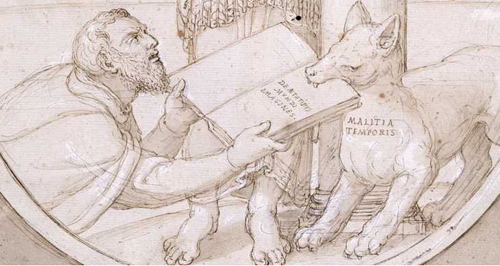
\includegraphics[height=0.3\textheight,keepaspectratio]
                          {images/malatia-temporis.png}
  \caption{Pormenor de um desenho de Franscisco da Holanda, ``O
    artista apresentando o seu livro''}
  \label{fig:3}
\end{figure}

Uma frase retirada da obra ``Da Pintura Antiga'' resume bem o tema
central do Desenho para Holanda:

\begin{quote}
  E em tanto ponho o Desenho, que me atraverei a mostrar como tudo o
  que se faz em este mundo é desenhar.
\end{quote}

O ``atrevimento'' de Holanda culmina precisamente na obra ``A ciência
do Desenho'', escrita mais de 20 anos depois da frase que a predizia.

Este atrevimento é curiosamente duplo: se por um lado a formulação
especulativa de Holanda é inovadora no campo do pensamento
estético-filosófico, por outro lado ela é ousada no facto de ser
endereçada directamente à pessoal real.

Se a abordagem às questões teológicas são feitas com certa delicadeza
e com socorro às emendas censura , o discurso à pessoal real assume um
tom claramente despreocupado, oscilando entre o ``queixume'' ou o
didatismo quase pedântico. Há ainda passagens satíricas: das ``grandes
nações'' que estimam o Desenho, somente Portugal ``que não sabe agora
mais disso que de coisa que nunca veio a sua notícia'', ``estima muito
qualquer outra coisa que pintura nem pintores''.

Ainda que, segundo Holanda, a sua intenção não seja a de ``abater os
entendimentos dos ínclitos e excelentíssimos Reis e Príncipes de
Portugal, porque me prezo de muito bom português'', pode especular-se
que esta postura só seria tolerada a alguém com certa confiança na
\emph{entourage} real, o que seria plausível dado que Holanda tinha
mantinha relações estreitas com D. João III, avô de D. Sebastião,
tendo viajado em seu serviço e inclusivé pintado dele um retrato.

Holanda nunca escamoteia o seu algum ressentimento. Refere, por
exemplo, que o seu espírito de artista se encontra ``de todo
arrefecido'' e que nele já morre ``o entendimento daquela ciência
[...] tão desestimada''. Diz-se esquecido ``em um Mato e Monte que
está entre Sintra e Lisboa'' e desaminado por não ``haver em que [...]
possa servir Vossa Alteza nem este reino''. É pouco provável que este
apelo tenha sido ouvido pelo seu destinatário. D. Sebastião viria a
escolher outros engenheiros para o acompanharem \cite[p.54]{holanda} e
perder-se-ia em Alcácer-Quibir, vítima certamente de uma campanha mal
desenhada.

Não deixa de ser curioso observar como, cerca de 1573, dois anos
depois de terminar ``A Ciência do Desenho'' e eventualmente o ter
apresentado ao Rei, Franscisco desenha um insólito auto-retrato para o
seu ``O Livro das Idades'', livro de o desenhos que o acompanhou
durante praticamente toda a vida e que Felipe II de Espanha, quem
Holanda terá ainda visto chegar ao trono de Português, viria a levar
para o Escorial de Madrid. No desenho, o artista apresenta o seu livro
a um cão furioso que o morde. No peito do cão, a inscrição ``malatia
temporis''.

\printbibliography[heading=bibliography,title={Bibliografia}]

\end{document}
